\documentclass{report}
\usepackage[showframe=false]{geometry}
\usepackage{titlesec}
\usepackage{amsmath}
\usepackage{graphicx}
\usepackage{float}

\pagenumbering{gobble}

\geometry{tmargin=60pt,bmargin=90pt,lmargin=90pt,
rmargin=90pt}

\titleformat{\chapter}{\normalfont\huge}{\thechapter.}{20pt}{\huge}
\titlespacing*{\chapter} {0pt}{0pt}{10pt}

\begin{document}

\chapter{Section 1}
\section{a.}

The vertebral column data was first read from the ARFF file, then split into classes for processing.

\begin{verbatim}
  library(foreign)
  vert <- read.arff("column_2C_weka.arff")
  vert_split <- split(vert, vert[,"class"])

  sapply(vert_split$Abnormal[0:6], mean)
  sapply(vert_split$Abnormal[0:6], median)
  sapply(vert_split$Abnormal[0:6], sd)
  sapply(vert_split$Normal[0:6], mean)
  sapply(vert_split$Normal[0:6], median)
  sapply(vert_split$Normal[0:6], sd)
\end{verbatim}

\subsection{Abnormal Data}

\begin{tabular}{l}
  mean \\
  \hskip 1.0cm\begin{tabular}{rrr}
    pelvic\_incidence & pelvic\_tilt & lumbar\_lordosis\_angle \\
    64.69256 & 19.79111 & 55.92537 \\
    sacral\_slope & pelvic\_radius & degree\_spondylolisthesis \\
    44.90145 & 115.07771 & 37.77771 \\
  \end{tabular} \\
  standard deviation \\
  \hskip 1.0cm\begin{tabular}{rrr}
    pelvic\_incidence & pelvic\_tilt & lumbar\_lordosis\_angle \\
    65.27489 & 18.79890 & 56.15000 \\
    sacral\_slope & pelvic\_radius & degree\_spondylolisthesis \\
    44.63960 & 115.65032 & 31.94652 \\
  \end{tabular} \\
  median \\
  \hskip 1.0cm\begin{tabular}{rrr}
    pelvic\_incidence & pelvic\_tilt & lumbar\_lordosis\_angle \\
    17.66213 & 10.51587 & 19.66947 \\
    sacral\_slope & pelvic\_radius & degree\_spondylolisthesis \\
    14.51556 & 14.09060 & 40.69674 \\
  \end{tabular}
\end{tabular}

\subsection{Normal Data}

\begin{tabular}{l}
  mean \\
  \hskip 1.0cm\begin{tabular}{rrr}
    pelvic\_incidence & pelvic\_tilt & lumbar\_lordosis\_angle \\
    0 & 0 & 0 \\
    sacral\_slope & pelvic\_radius & degree\_spondylolisthesis \\
    0 & 0 & 0 \\
  \end{tabular} \\
  standard deviation \\
  \hskip 1.0cm\begin{tabular}{rrr}
    pelvic\_incidence & pelvic\_tilt & lumbar\_lordosis\_angle \\
    0 & 0 & 0 \\
    sacral\_slope & pelvic\_radius & degree\_spondylolisthesis \\
    0 & 0 & 0 \\
  \end{tabular} \\
  median \\
  \hskip 1.0cm\begin{tabular}{rrr}
    pelvic\_incidence & pelvic\_tilt & lumbar\_lordosis\_angle \\
    0 & 0 & 0 \\
    sacral\_slope & pelvic\_radius & degree\_spondylolisthesis \\
    0 & 0 & 0 \\
  \end{tabular}
\end{tabular}

\section{b.}

\begin{verbatim}
  library(foreign)
  vert <- read.arff("column_2C_weka.arff")
\end{verbatim}

\begin{figure}[h!]
  \includegraphics[width=\linewidth]{ImageNameHere.png}
  \caption{Caption Here}
  \label{fig:LabelHere}
\end{figure}

\section{c.}

\chapter{Section 2}

\section{a.}

Generating 100 3-dimensional vectors from a normal disribution with a mean vector as [1 2 1] and a 3x3 covariance matrix as [4  0.8 -0.3; 0.8 2 0.6; -0.3 0.6 5]

\begin{verbatim}
  mean <- c(1,2,1)
  sigma <- matrix(c(4, 0.8, -0.3, 0.8, 2, 0.6, -0.3, 0.6, 5), 3,3)
\end{verbatim}

\[
  mean <-
  \begin{bmatrix}
    1 & 2 & 1
  \end{bmatrix}
\]

\[
  sigma <-
  \begin{bmatrix}
    4 & 0.8 & -0.3 \\
    0.8 & 2 & 0.6 \\
    -0.3 & 0.6 & 5
  \end{bmatrix}
\]

\section{b.}

\begin{figure}[H]
  \includegraphics[width=\linewidth]{ImageNameHere.png}
  \caption{Caption Here}
  \label{fig:LabelHere}
\end{figure}

\section{c.}

\begin{verbatim}
  library(fields)
  Euclidean <- rdist(x1, x2)
\end{verbatim}

\[
  x1 <-
  \begin{bmatrix}
    0 & 0 & 0
  \end{bmatrix}
\]

\[
  x2 <-
  \begin{bmatrix}
    0 & 0 & 0
  \end{bmatrix}
\]

\[
  Euclidean <-
  \begin{bmatrix}
    0
  \end{bmatrix}
\]

\begin{verbatim}
  library(stats)
  Mahalanobis<-mahalanobis(x,mean,cov) 
\end{verbatim}

\[
  x <-
  \begin{bmatrix}
  \end{bmatrix}
\]

\[
  mean <-
  \begin{bmatrix}
  \end{bmatrix}
\]

\[
  cov <-
  \begin{bmatrix}
  \end{bmatrix}
\]

\[
  Mahalanobis <-
  \begin{bmatrix}
  \end{bmatrix}
\]



\chapter{Section 3}

\section{Eigenvalues \& Eigenvectors}

\begin{verbatim}
	records <- read.table("five-dimensional-records.txt")
  mean <- colMeans(records)
	cov <- cov(records)
\end{verbatim}

\[
  mean <- 
  \begin{bmatrix}
  \end{bmatrix}
\]

\[
  cov <- 
  \begin{bmatrix}
  \end{bmatrix}
\]

\begin{verbatim}
\end{verbatim}

\[
  Eigenvalues <- 
  \begin{bmatrix}
  \end{bmatrix} \\
\]

\[
  Eigenvectors <- 
  \begin{bmatrix}
  \end{bmatrix}
\]

\begin{figure}[H]
  \includegraphics[width=\linewidth]{ImageNameHere.png}
  \caption{Caption Here}
  \label{fig:LabelHere}
\end{figure}

\section{reduced representation}

\begin{verbatim}	
\end{verbatim}

\[
  PCA <- 
  \begin{bmatrix}
  \end{bmatrix}
\]

\section{Scatter Plot}

\begin{figure}[H]
  \includegraphics[width=\linewidth]{ImageNameHere.png}
  \caption{Caption Here}
  \label{fig:LabelHere}
\end{figure}

\section{Reconstruct Data}

\begin{verbatim}	
\end{verbatim}

\[
  records <- 
  \begin{bmatrix}
    5700 & 12.8 & 2500 & 270 & 25000 \\
    1000 & 10.9 & 600 & 10 & 10000 \\
    3400 & 8.8 & 1000 & 10 & 9000 \\
    3800 & 13.6 & 1700 & 140 & 25000 \\
    4000 & 12.8 & 1600 & 140 & 25000 \\
    8200 & 8.3 & 2600 & 60 & 12000 \\
    1200 & 11.4 & 400 & 10 & 16000 \\
    9100 & 11.5 & 3300 & 60 & 14000 \\
    9900 & 12.5 & 3400 & 180 & 18000 \\
    9600 & 13.7 & 3600 & 390 & 25000 \\
    9600 & 9.6 & 3300 & 80 & 12000 \\
    9400 & 11.4 & 4000 & 100 & 13000
  \end{bmatrix}
\]

\[
  reconstructed <- 
  \begin{bmatrix}
  \end{bmatrix}
\]

\[
  sqareerr <- 
  \begin{bmatrix}
  \end{bmatrix}
\]

\chapter{Section 4}

\begin{verbatim}	
\end{verbatim}

\[
  Eigenvalues <- 
  \begin{bmatrix}
  \end{bmatrix}
\]

\[
  Eigenvectors <- 
  \begin{bmatrix}
  \end{bmatrix}
\]

\begin{figure}[H]
  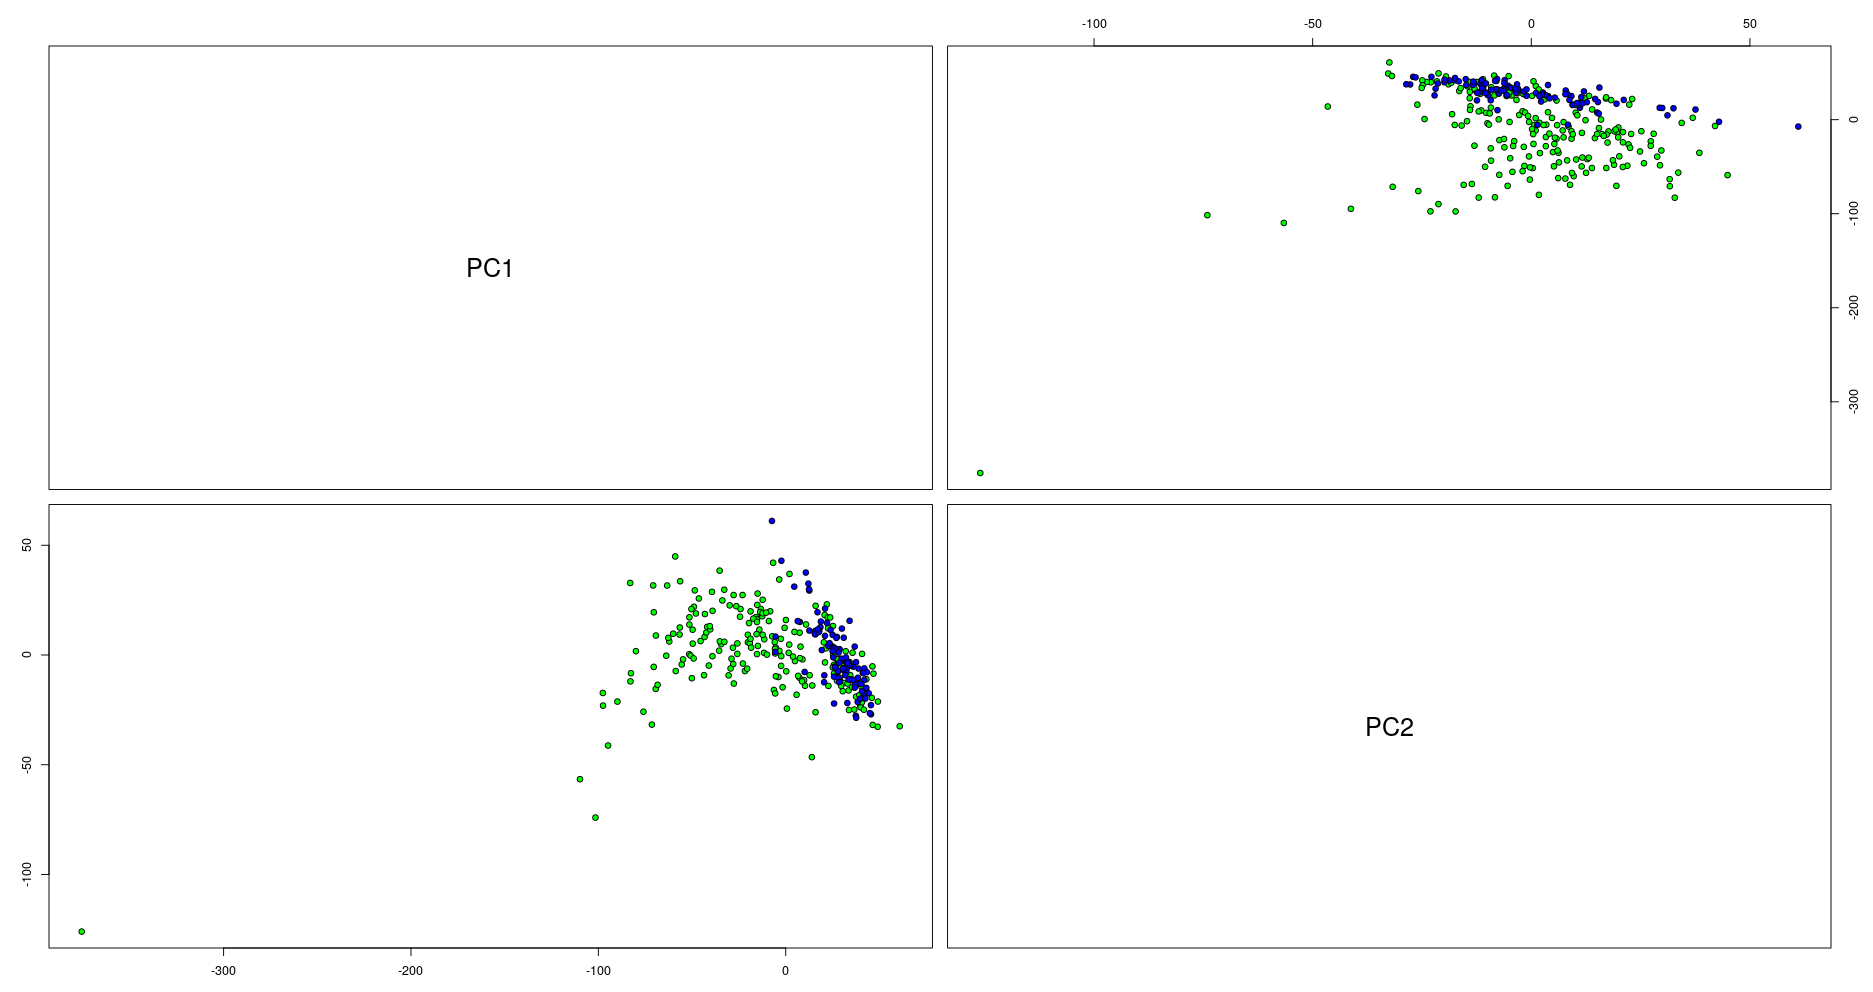
\includegraphics[width=\linewidth]{pca_vertebral_column_data_set.png}
  \caption{PCA Vertebral Column Data Set}
  \label{fig:PCAVertebralColumnDataSetScatterPlot}
\end{figure}

\chapter{Section 5}

\begin{verbatim}	
  library('tsne')
  records <- read.table('five-dimensional-records.txt') 
  tsne_10 <- tsne(records, perplexity=10)
  tsne_50 <- tsne(records, perplexity=50)
\end{verbatim}

\[
  tsne\_10 <- 
  \begin{bmatrix}
  \end{bmatrix}
\]

\[
  tsne\_50 <- 
  \begin{bmatrix}
  \end{bmatrix}
\]

\begin{figure}[H]
  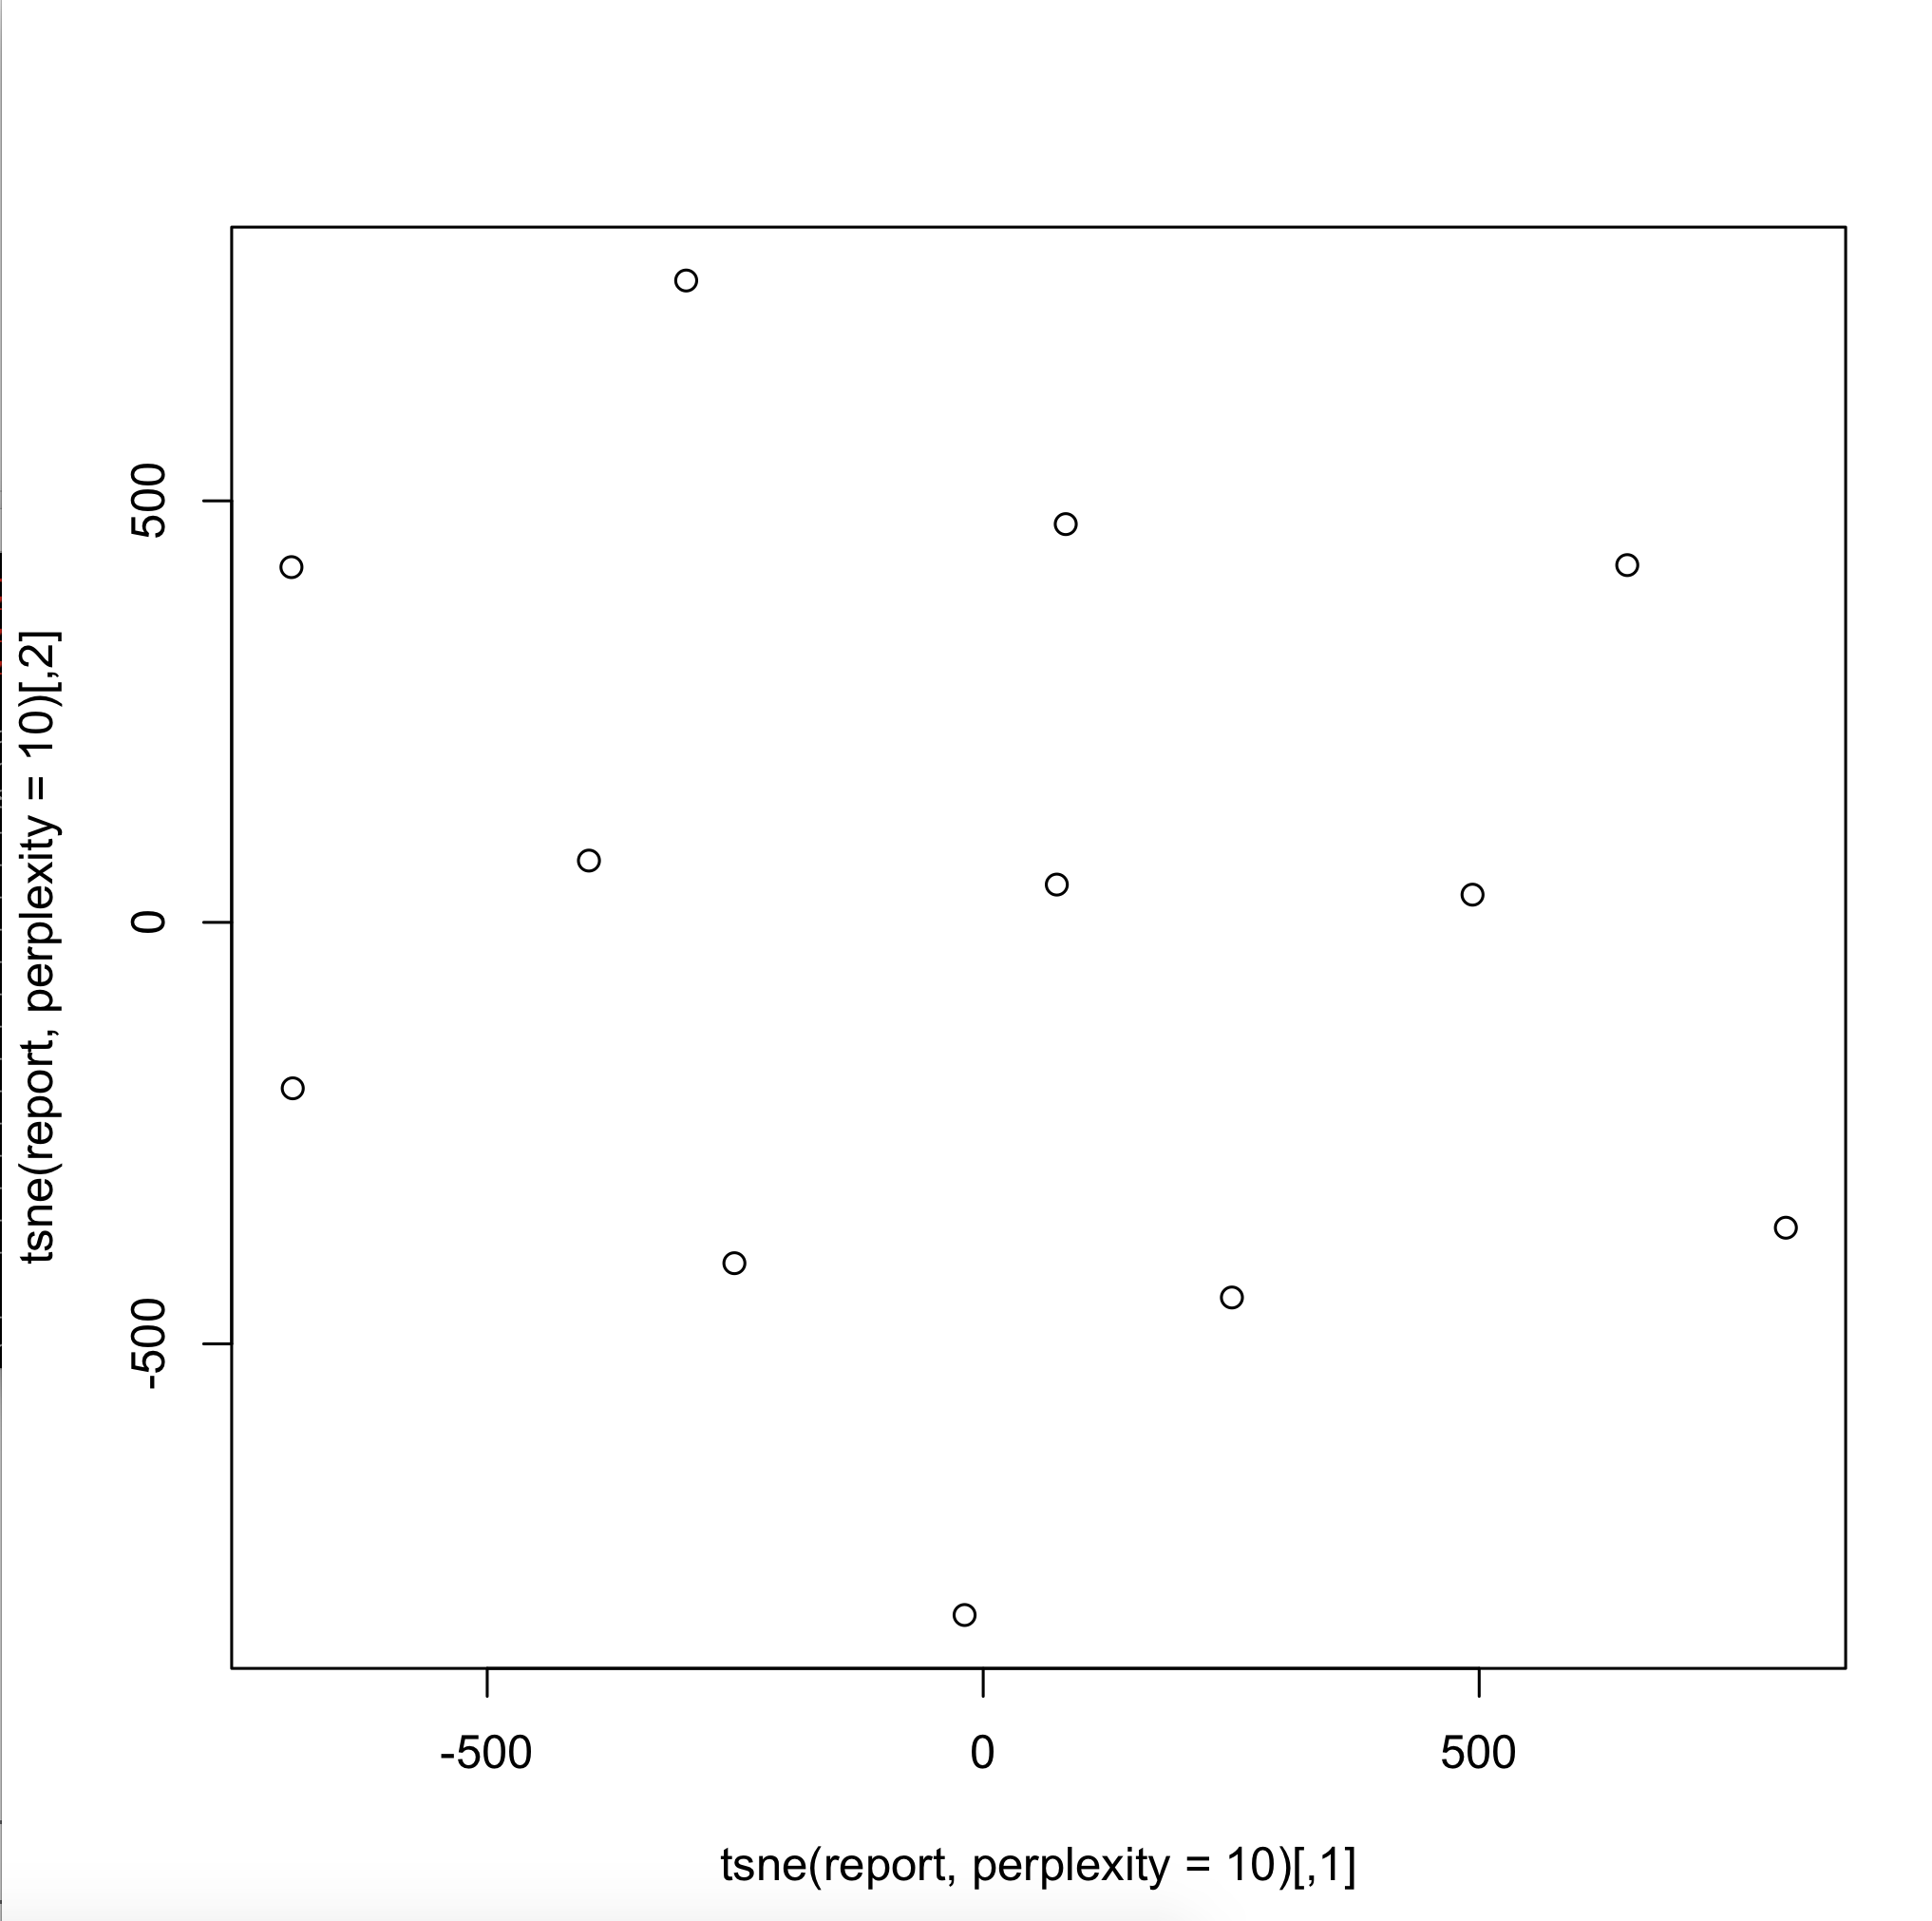
\includegraphics[width=\linewidth]{tsne_p_10.png}
  \caption{tsne perplexity 10}
  \label{fig:tsnep10}
\end{figure}

\begin{figure}[H]
  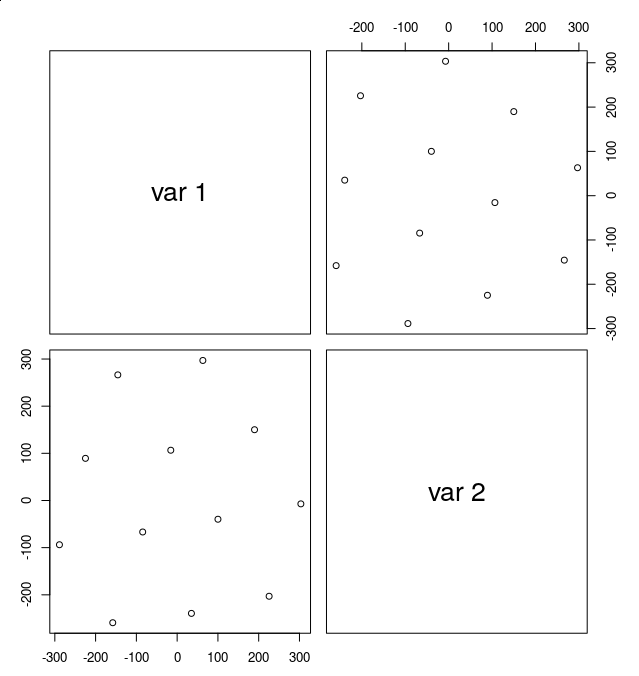
\includegraphics[width=\linewidth]{tsne_p_50.png}
  \caption{tsne perplexity 50}
  \label{fig:tsnep50}
\end{figure}

\end{document}







































